\section{Metodología de trabajo propuesta}
Este trabajo consiste principalmente en la recolección de datos que posteriormente deben pasar por distintas etapas tales como análisis, organización, clasificación y, en algunos casos, normalización. Una vez se haya logrado el entendimiento de los datos se procede a establecer una serie de funciones matemáticas de estimación y/o regresión, y posteriormente un modelo dinámico mediante ecuaciones diferenciales. Finalmente, este modelo deberá ser evaluado para verificar si éste puede estimar variables de manera apropiada.\\

Teniendo en cuenta las etapas principales anteriormente mencionadas, y teniendo en consideración la literatura disponible para proyectos de este tipo; se considera plausible proponer una adaptación de la metodología CRISP-DM, a los intereses del proyecto. 
%La metodología CRISP-DM es descrita a continuación:


\section{Metodología CRISP-DM}\label{crispmethod}

\begin{figure}[H]
    \centering
    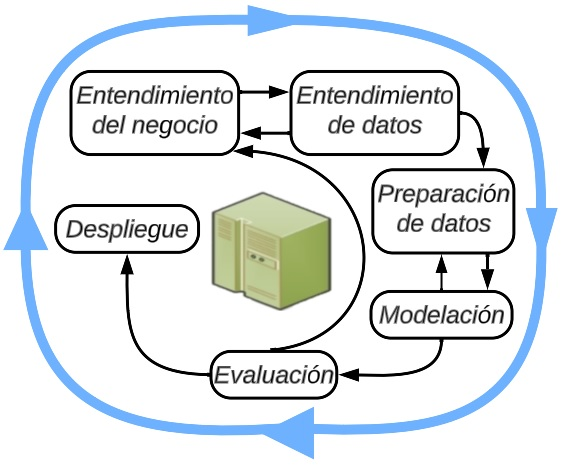
\includegraphics[scale=0.50]{img/ciclocrispspa.jpg}
    \caption{Ciclo de Vida de minería de datos. Modificada de \cite{ibmcrisp}.}
    \label{ciclocrisp}
\end{figure}


La metodología CRISP-DM, por sus siglas en Inglés, Cross Industry Standar Process for Data Mining, propone un método probado para orientar trabajos de minería de datos. Puede ser abarcada de 2 maneras; como proceso, ofreciendo un resumen del ciclo vital de la minería de datos; y como una metodología, en la que se incluye descripciones de las fases normales de un proyecto, incluyendo las tareas necesarias de cada etapa y una explicación inter-relacional entre las tareas \cite{ibmcrisp}.\\


Una de las características de esta metodología es su flexibilidad y personalización de un modelo de minería de datos que se adapte a las necesidades del proyecto. Esta metodología cuenta con un ciclo de vida compuesto por 6 fases o etapas no necesariamente secuenciales; y es en estas etapas donde se indican las dependencias más importantes y frecuentes entre las fases \cite{ibmcrisp}.



Tal y como se observa en la Figura \ref{ciclocrisp}, las etapas de la metodología son:





\subsection{Entendimiento del negocio} 
Esta primera etapa consiste principalmente en obtener la máxima cantidad de información posible de los objetivos comerciales. De esta forma se puede identificar de manera clara los objetivos, metas, problemas, y recursos con los que se cuentan para realizar el estudio. La metodología sugiere la recopilación de información sobre la situación comercial actual, los recursos personales, materiales e intangibles. Por otra parte se debe tener claro conocimiento de la estructura de la empresa, patrocinadores internos o externos y unidades comerciales que se verán afectadas positiva o negativamente tras la realización del proyecto de minería de datos \cite{ibmcrisp}.

\subsection{Entendimiento de los datos}
Esta etapa implica estudiar más de cerca los datos disponibles de minería. Esto es un paso imprescindible para evitar problemas inesperados durante la fase de preparación de datos pues suele ser la más larga en los proyectos \cite{ibmcrisp}.\\

En esta etapa se busca acceder a los datos, explorarlos mediante tablas, gráficos o análisis estadísticos. De esta forma se podrá determinar la calidad de los datos y describir resultados en la documentación del proyecto.

En este punto de la metodología se puede catalogar los datos de 3 maneras distintas
\begin{itemize}
    \item Datos existentes: registros, transacciones, encuesta, registro web, entre otros
    \item Datos adquiridos: Datos adicionales que pueden ser, o no, necesario incluirlos.
    \item Datos adicionales:Datos complementarios si los requiere
\end{itemize}
Con base en lo anterior y con las delimitaciones de la Sección \ref{limites}, se puede establecer que para este proyecto se trabajará principalmente con los datos existentes. También es importante realizar una descripción detallada de los datos, ya sea en cantidad o calidad; tipos de valores, ya sean numéricos, categóricos o booleanos; esquemas de codificación

\subsection{Preparación de los datos}
La preparación de datos es uno de los aspectos más importantes pues se busca que los datos cuenten con una estructura indicada para que los modelos que se propongan pueden satisfacer las necesidades para los que son propuestos. Es posible que para llevar a cabo esta etapa se deba realizar una combinación o agrupación de datos o registros, realizar una selección de muestra de un subconjunto de datos, agregación de registros, clasificación de datos para el modelado, eliminación y/o sustitución de valores en blanco o perdidos, ó la división en conjuntos de datos de prueba, entrenamiento o evaluación \cite{ibmcrisp}.\\

En cuanto a la selección de datos, es necesario que los datos sean relevantes por lo que se pueden seleccionar datos basados en la selección de elementos (filas de registros) o en la selección de atributos (columnas o características). Posteriormente a esto se debe realizar una limpieza de datos en donde se debe tratar con datos perdidos o en blanco, metadatos erróneos o perdidos, incoherencias y errores de datos, en cuyo caso deben ser corregidos \cite{ibmcrisp}.



\subsection{Modelación} 

Este es el punto donde los datos preparados pueden incorporarse a las herramientas analíticas y cuyos resultados podrán arrojar primeros resultados deseados respecto al problema planteado en la comprensión del negocio. El modelado se suele ejecutar en múltiples iteraciones. Normalmente, los analistas de datos ejecutan varios modelos utilizando los parámetros predeterminados y ajustan los parámetros o vuelven a la fase de preparación de datos para las manipulaciones necesarias por su modelo. Es necesario que el modelo sea acorde a los tipos de datos disponibles, a los objetivos y patrones, y a los requisitos específicos de modelado como por ejemplo si se busca que los resultados sean fácilmente presentables.\\

En cuanto a la generación de los modelos es necesario dedicar el tiempo suficiente para experimentar con distintos modelos antes de llegar a conclusiones definitivas. Estos modelos pueden ofrecer resultados interesantes en cuanto a interpretaciones y conclusiones. También puede realizarse una comparativa de modelos antes de integrarlos o desplegarlos. Para registrar el proceso con una amplia variedad de modelos es necesario asegurarse de registrar los cambios que se realicen en cada modelo en pro de corroborar y/o analizar los resultados cuando sea necesario.

Al final de esta etapa se dispondrá de 3 tipos de información que pueden ser usados para la toma de decisiones posteriores; estos datos son: 
\begin{enumerate}
    \item Configuración de parámetros donde se incluyen las notas que se han tomado sobre los parámetros que ofrecen mejores resultados.
    \item Los modelos producidos.
    \item Las descripciones de resultados de los modelos, incluyendo resultados asociados a problemas con los datos, rendimiento y exploración de resultados
\end{enumerate}

% \subsubsection{Modelamiento por Ecuaciones Diferenciales Ordinarias (EDOs)}

% \subsubsection{Modelamiento EDO: Balance de energía}


\subsection{Evaluación} 

En este punto, se habrá completado la mayor parte del proyecto. También se habrá determinado, en la fase de modelado, que los modelos son técnicamente correctos y efectivos en función de los objetivos que se han definido previamente. Esta etapa de la metodología produce 2 tipos de resultados: \begin{itemize}
    \item Los modelos finales seleccionados en la fase anterior de CRISP-DM.
    \item Las conclusiones o inferencias obtenidas de los modelos y del proceso de minería de datos; recibiendo el nombre de \textit{\textbf{descubrimientos}}.
\end{itemize}

Es en esta etapa donde se debe verificar si los resultados se expresan con claridad y de forma que se pueden representar con facilidad; si se han realizado descubrimientos especiales o particularidades que se deban resaltar; y si los resultados se adaptan a los objetivos del proyecto. Una vez haya evaluado los resultados, es recomendable realizar una lista de el (los) modelo(s) aprobado(s) para incluir en el informe final.


\subsection{Despliegue} 
En general, la fase de despliegue de CRISP-DM incluye dos tipos de actividades:
\begin{itemize}
    \item Planificación y control del despliegue de los resultados
    \item Finalización de tareas de presentación como la producción de un informe final y la revisión del proyecto
\end{itemize}
